\chapter{Organisation}
\label{ch:Organisation}

\section{Zeitplanung und Aktivitäten}
Die Bearbeitung der Bachelorarbeit soll maximal vier Monate (von März bis Juli) dauern und erfolgt in mehreren Arbeitsschritten, die wir im Folgenden definieren. Der zeitliche Ablauf ist in der Abbildung \ref{fig:arbeitsschritte} dargestellt.

\begin{figure}[h]
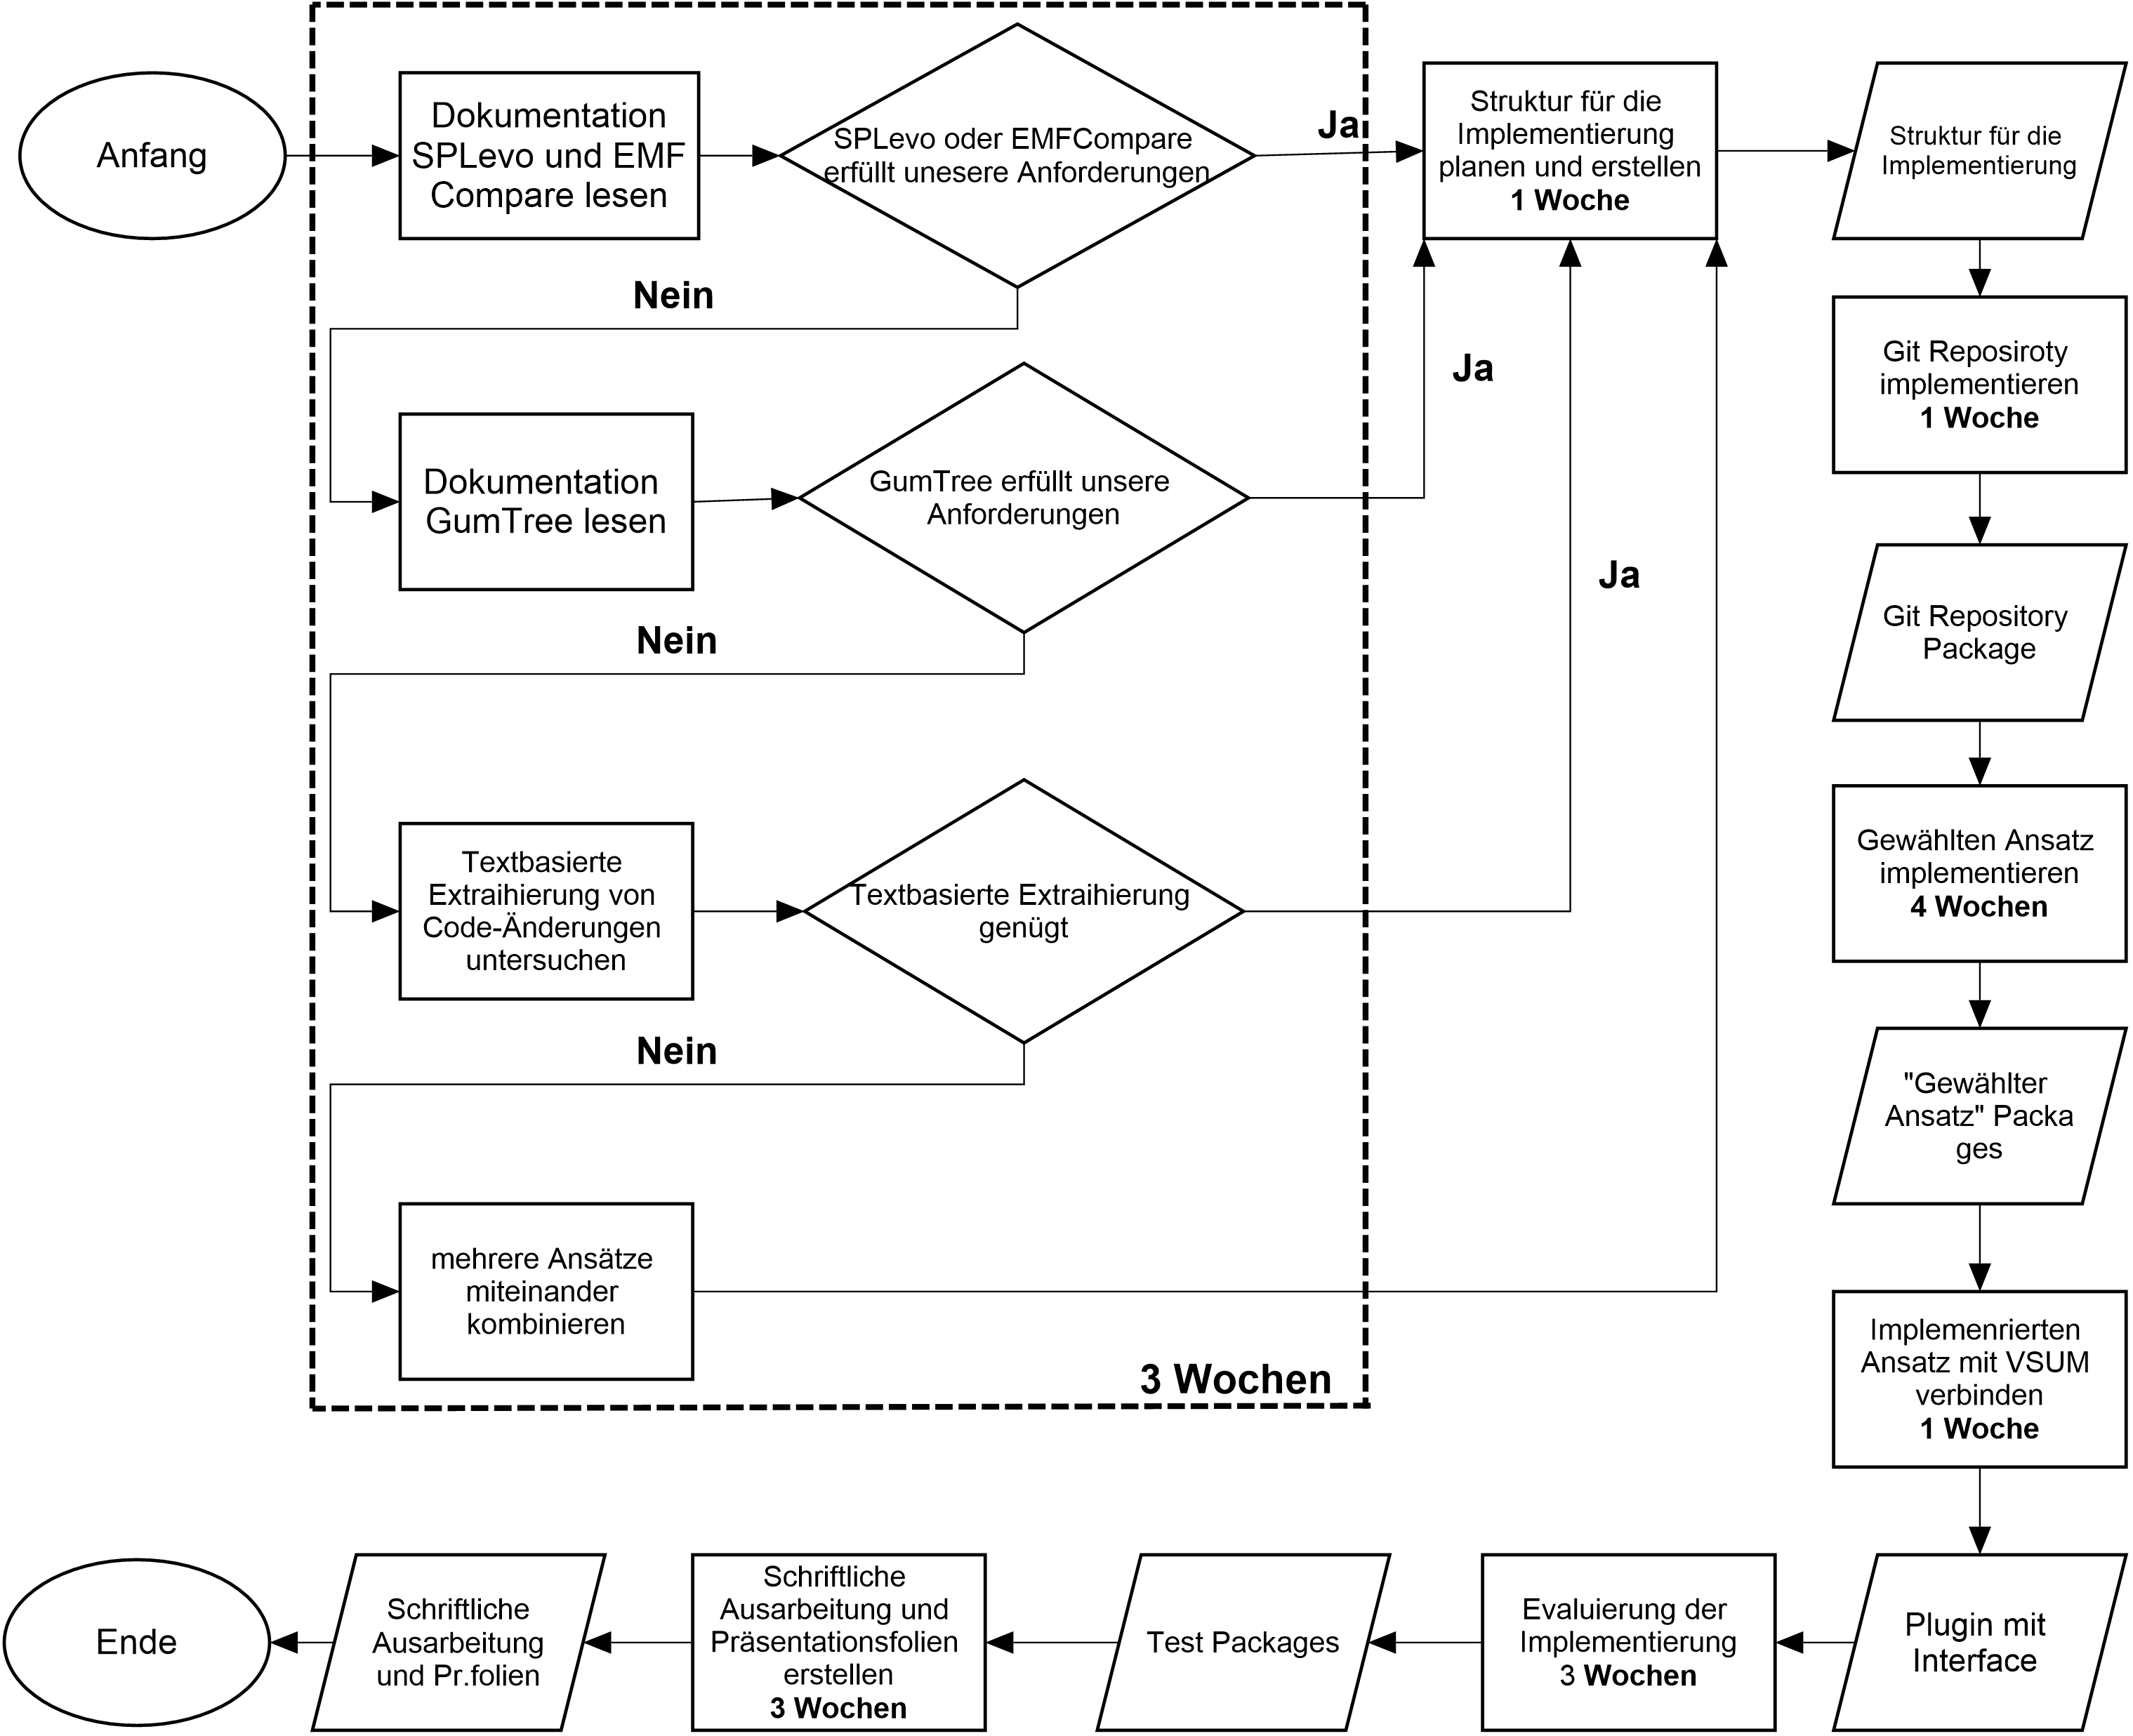
\includegraphics[width=\textwidth]{pictures/Zeitplan.png}
\caption{Bearbeitungsplan für die Bachelorarbeit mit Zeitangaben. Ein Rechteck bezeichnet einen Prozess, ein Parallelogramm eine Ein-/Ausgabe, eine Raute eine Entscheidung}
\label{fig:arbeitsschritte}
\end{figure}

\subsection{Lesen von Dokumentation und Durchführung kleiner Experimente}
Zuerst wollen wir uns auf den dritten Ansatz aus dem Kapitel 'Konzeption' konzentrieren. In dem Ansatz müssen wir JaMoPP-Modelle \cite{jamopp} mithilfe von SPLevo \cite{splevo}oder EMF Compare \cite{emfcompare} miteinander vergleichen. Dafür müssen wir die Dokumentationen von SPLevo und EMF Compare genauer lesen. Da diese sehr umfangreich sein können, konzentrieren wir uns dabei auf die für uns relevanten Funktionalitäten. Gegebenenfalls führen wir auch kleine Experimente, um zu entscheiden, ob/welches von beiden Tools wir für unsere Implementierung benutzen. Falls keins von beiden unsere Anforderungen erfüllt, werden wir auf gleiche Art den zweiten Ansatz aus dem Kapitel 'Konzeption' \ref{ch:Konzeption} untersuchen. Falls uns auch dieser Ansatz nicht passt, entscheiden wir uns entweder für den ersten Ansatz aus dem Kapitel 'Konzeption' \ref{ch:Konzeption} oder für eine Kombination von mehreren Ansätzen. Über eine genaue Vorgehensweise sowie gegebenenfalls ein Verzicht auf manche geplanten Funktionalitäten wird in diesem Fall mit dem wissenschaftlichen Betreuer diskutiert.

\subsection{Planung und Erstellung einer Struktur für die Implementierung}
In diesem Schritt erstellen wir eine Struktur für unsere Implementierung. Wir definieren (soweit möglich) alle nötigen Projekte, Packages, Klassen und Methoden.

\subsection{Implementierung eines Git-Repository}
In dem Kapitel Konzeption \ref{ch:Konzeption} haben wir drei Ansätze vorgestellt, wie die Behandlung eines Commits und darauf folgende Aktualisierung von einem JaMoPP-Modells durchgeführt werden kann. Unabhängig von dem gewählten Ansatz muss zuerst das Commit ausgelesen und zwischengespeichert werden. Dafür implementieren wir ein Package, das ein Git-Repository darstellt. Wir benutzen JGit \cite{jgit} als Hilfsbibliothek.  Das implementierte Git-Repository speichert die ankommenden Commits und unterteilt jedes Commit in einzelne Differenzen (Diffs).

\subsection{Implementierung des gewählten Ansatzes}
In diesem Schritt implementieren wir den gewählten Ansatz. Der Ansatz soll als Eingabe ein Commit erhalten. Das Commit soll in dem im vorherigen Schritt implementierten Repository gespeichert und vorverarbeitet werden. Für jedes Java-File, wo Änderungen stattfinden, müssen wir diese Änderungen in dem korrespondierenden JaMoPP-Modell anwenden. Das heißt, das JaMoPP-Modell muss anhand von den Änderungen im Java-Quellcode aktualisiert werden. Am Ende dieses Schrittes sollen alle nötigen Funktionalitäten implementiert sein, die es ermöglichen, anhand von Quellcode-Änderungen das existierende JaMoPP-Modell zu aktualisieren.

\subsection{Verbinden des implementierten Ansatzes mit VSUM}
Alle erstellen Modellen werden in Vitruvius in einem Virtual Signle Underliyng Model (VSUM) \ref{sec:Vitruvius} gespeichert, darunter auch JaMoPP-Modelle. Deshalb müssen wir unseren implementierten Ansatz mit VSUM verbinden. Dafür erstellen wir ein Eclipse Plugin mit einem entsprechenden Interface.  

\subsection{Evaluierung}
In der Evaluierung unseres Ansatzes wollen wir zwei Aspekte überprüfen. Als erstes wollen wir zeigen, dass JaMoPP-Modelle richtig aktualisiert werden. Anschließend wollen wir unseren Ansatz in den CIPM-Ansatz \ref{sec:Continuous Integration of Performance Model} integrieren und überprüfen, ob auch SEFFs \ref{sec:Palladio Component Model} richtig aktualisiert werden. Eine genauere Vorgehensweise wurde in dem Kapitel \ref{ch:Konzeption} beschrieben.
%Für die Evaluierung der implementierten Funktionalitäten importieren wir ein Open Source Project und die zu ihm gehörenden Commits. Für jedes Java-File erstellen wir ein JaMoPP-Modell und fügen es zu dem VSUM. Für jedes vorhandene Commit ermitteln wir die von den Änderungen betroffen Java-Files, finden ihre korrespondierenden JaMoPP-Modelle in VSUM und aktualisieren sie. Dann wenden wir die Änderungen auf den Java-Quellcode an und erstellen von diesen aktualisierten Java-Files neue JaMoPP-Modelle.  Anschließend vergleichen wir die neu erstellten JaMoPP-Modelle mit den entsprechenden aktualisierten JaMoPP-Modellen. Wenn unsere Implementierung korrekt ist, soll der Vergleich keine Unterschiede zwischen den neuen und den aktualisierten JaMoPP-Modellen finden.


\section{Risikomanagement}
In dieser Bachelorarbeit werden viele zusätzlichen Software-Tools eingesetzt. Manche von diesen sind wissenschaftliche Projekte, die noch nicht komplett implementiert oder fehlerfrei sind. Einige Projekte werden nicht mehr oder nur selten aktualisiert. Das kann zu den Kompatibilitätsproblemen führen oder die Ausführbarkeit der von uns implementierten Funktionalität verhindern oder einschränken. Falls solche Probleme auftreten, können wir folgende Auswege nehmen:
\begin{itemize}
\item Funktionalität unserer Implementierung einschränken
\item Andere Software-Tools und Bibliotheken benutzen statt der geplanten
\item Falls wir uns auf keiner fortgeschrittenen Etappe in unserer Implementierung befinden, greifen wir zu einem anderen von den drei vorgestellten Ansätzen oder kombinieren diese Ansätze miteinander
\end{itemize}
In jeder geplanten Arbeitsphase kann es zu einem zeitlichen Verzug kommen. Mögliche Gründe dafür sind zum Beispiel eine Krankheit, keine oder mangelnde Erfahrung mit den eingesetzten Software-Tools und Bibliotheken oder fehlerhaftes Verhalten von diesen. Deshalb werden die letzte Woche in dem Zeitplan als Puffer frei gehalten. Außerdem kann eine Fristverlängerung der Bearbeitungszeit um einen Monat beantragt werden. Im Notfall muss nach der Absprache mit dem wissenschaftlichen Betreuer auf Implementierung einiger geplanter Funktionen verzichtet werden.  
